\subsection{Extraction de séquences}

Pour cette première partie, seulS quelques extraits de code seront présentés. L'intégralité du code source se trouve dans le fichier \texttt{src/hmmPart1.r} du projet. 

\subsubsection*{Extension de la fonction \texttt{simu\_symbol}}

La fonction \texttt{simu\_symbol} permet de construire et d'afficher des chiffres. Pour cela, elle récupère un ensemble de 30 points différents, qu'elle relie ensuite dans un odre précis. L'extension de cette fonction par le code ci-dessous, permet désormais de construire le chiffre 6.

\begin{lstlisting}
simu_symbol <- function()
{
	(...)
	digit_6 <- rbind(
		stroke(-0.5,1.0,-0.5,-0.5,10),
		stroke(-0.4,-0.5,0.5,-0.5,7),
		stroke(0.5,-0.4,0.5,0.4,6),
		stroke(0.4,0.4,-0.5,0.4,7)
	)
  dimnames(digit_6) <- list(num=1:nrow(digit_6),point=c("x","y"))
  plot(digit_6,type="l",col="red",xlim=c(-1,1),ylim=c(-1,1))
  points(digit_6)
  return(list(d1=digit_1,d2=digit_4,d3=digit_6))
}
\end{lstlisting}

\subsubsection*{Analyse de la fonction \texttt{compute\_symbol}}
La fonction \texttt{compute\_symbol} prend trois paramètres en entrée : le tracé d'un chiffre, un nombre de lignes (5) et un nombre de colonnes (3). Elle commence par construire une matrice, ayant pour dimension le nombre de lignes et de colonnes précisés précédemment. Cette matrice servira à positionner les points du tracé analysé :
\begin{center}
	$\begin{pmatrix}
		13 & 14 & 15 \\
		10 & 11 & 12 \\
		7 & 8 & 9 \\
		4 & 5 & 6 \\
		1 & 2 & 3
	\end{pmatrix}$
\end{center}

Elle calcule ensuite le nombre de points présents dans le tracé du chiffre, puis les positions horizontales et verticales de chacun de ces points. Pour finir, elle détermine la position de chaque point dans la matrice qu'elle a créée, et les affiche.\\

Voici les résultats donnés par cette fonction pour les trois tracés créés par la fonction \texttt{simu\_symbol} :
\begin{lstlisting}
	pour 1 : 11 11 14 14 14 14 14 14 14 14 14 14 14 14 11 11 11 11 8 8 8 8 5 5 5 5 2 2 2 2 
	pour 4 : 14 14 14 11 11 10 7 7 7 4 4 4 4 4 5 8 8 8 9 9 8 8 8 5 5 5 2 2 2 2 
	pour 6 : 13 13 13 10 10 7 7 7 4 4 4 5 5 5 5 6 6 6 6 9 9 12 12 12 11 11 11 11 10 10 
\end{lstlisting}
Ce qui donne pour le chiffre "6", les positions suivantes :
\begin{center}
	$\begin{pmatrix}
		 \textcolor{red}{13} & 14 & 15 \\
		\textcolor{red}{10} & \textcolor{red}{11} & \textcolor{red}{12} \\
		\textcolor{red}{7} & 8 & \textcolor{red}{9} \\
		\textcolor{red}{4} & \textcolor{red}{5} & \textcolor{red}{6} \\
		1 & 2 & 3
	\end{pmatrix}$
\end{center}

Avec une matrice contenant suffisamment de lignes et de colonnes, cette méthode permet de déterminer efficacement la position de chaque point d'un caractère. Cependant, si le caractère analysé est mal positionné (décalage à gauche ou à droite), toutes les positions sont également décalées au niveau de la matrice. Il faut donc faire un traitement important en amont pour que le caractère soit bien découpé et bien positionné. De plus, l'ordre de chaque point est essentiel pour la construction de la séquence.

\subsubsection*{Analyse de la fonction \texttt{compute\_symbol\_dir}}
La fonction \texttt{compute\_symbol\_dir} prend deux paramètres en entrée : le tracé d'un chiffre et un nombre d'angles qui serviront de direction (ici 8). Chaque direction est numérotée telle que :
\begin{center}
	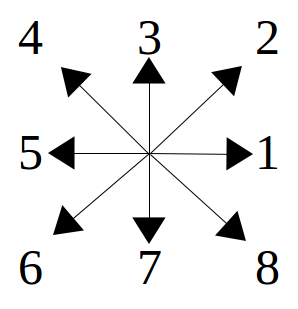
\includegraphics[width=0.20\textwidth]{Figures/direction.jpg}
\end{center}
Ainsi, la direction 1 indique un déplacement vers la droite, la direction 5 vers la gauche, etc\dots \\

Voici les résultats donnés par cette fonction pour les trois tracés créés par la fonction \texttt{simu\_symbol\_dir} :
\begin{lstlisting}
	pour 1 : 2 2 2 2 2 2 2 2 2 7 7 7 7 7 7 7 7 7 7 7 7 7 7 7 7 7 7 7 7 7 
	pour 4 : 6 6 6 6 6 6 6 6 6 5 1 1 1 1 1 1 1 1 1 4 7 7 7 7 7 7 7 7 7 7 
	pour 6 : 7 7 7 7 7 7 7 7 7 1 1 1 1 1 1 1 3 3 3 3 3 3 5 5 5 5 5 5 5 5 
\end{lstlisting}
Ce qui donne pour le chiffre "1" deux tracés : le premier allant vers le 2 et le second allant vers le 7.
\begin{center}
	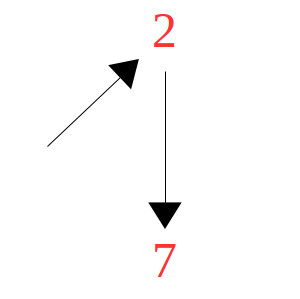
\includegraphics[width=0.20\textwidth]{Figures/direction_results.jpg}
\end{center}

L'un des principaux avantages de cette méthode est que la taille de la séquence, ainsi que sa position (avec ou sans décalage) n'affectent pas les résultats. Cette fonction arrive à déterminer précisément l'angle de la direction du tracé. Cependant, si l'image n'est pas dans le bon sens ou si l'écriture est inclinée ou en italique, la reconnaissance de l'angle sera faussée. De plus, le chiffre "1" et le chiffre "7" peuvent être facilement confondus à cause de certaines polices d'écriture. L'ordre de chaque point est également essentiel pour la construction de la séquence.


\subsection{Création et initialisation d'un HMM}

Pour cette nouvelle partie, nous considérerons un HMM à 3 états ($S_x$), observant 10 chiffres ($c_x$) et une topologie gauche-droite :
\begin{center}
	\begin{tikzpicture}
	 	% states
		\node[state] (s1) at (1,2) {$S_1$}
			edge [loop above] node[auto] {0.9} ();
		\node[state] (s2) at (4.5,2) {$S_2$}
			edge [<-,bend left=0] node[auto] {0.1} (s1)
			edge [loop above] node[auto] {0.9} ();
		\node[state] (s3) at (8,2) {$S_3$}
			edge [<-,bend left=0] node[auto] {0.1}  (s2)
			edge [loop above] node[auto] {1} ();
		% observations
		\node[observation] (c0) at (0,0) {$c_0$}
			edge [lightedge] (s1)
			edge [lightedge] (s2)
			edge [lightedge] (s3);
		\node[observation] (c1) at (1,0) {$c_1$}
			edge [lightedge] (s1)
			edge [lightedge] (s2)
			edge [lightedge] (s3);
		\node[observation] (c2) at (2,0) {$c_2$}
			edge [lightedge] (s1)
			edge [lightedge] (s2)
			edge [lightedge] (s3);
		\node[observation] (c3) at (3,0) {$c_3$}
			edge [lightedge] (s1)
			edge [lightedge] (s2)
			edge [lightedge] (s3);
		\node[observation] (c4) at (4,0) {$c_4$}
			edge [lightedge] (s1)
			edge [lightedge] (s2)
			edge [lightedge] (s3);
		\node[observation] (c5) at (5,0) {$c_5$}
			edge [lightedge] (s1)
			edge [lightedge] (s2)
			edge [lightedge] (s3);
		\node[observation] (c6) at (6,0) {$c_6$}
			edge [lightedge] (s1)
			edge [lightedge] (s2)
			edge [lightedge] (s3);
		\node[observation] (c7) at (7,0) {$c_7$}
			edge [lightedge] (s1)
			edge [lightedge] (s2)
			edge [lightedge] (s3);
		\node[observation] (c8) at (8,0) {$c_8$}
			edge [lightedge] (s1)
			edge [lightedge] (s2)
			edge [lightedge] (s3);
		\node[observation] (c9) at (9,0) {$c_9$}
			edge [lightedge] (s1)
			edge [lightedge] (s2)
			edge [lightedge] (s3);
	\end{tikzpicture}
\end{center}

Pour ce HMM observant une topologie gauche-droite, il est nécessaire que l'état $S_1$ soit l'état initial. Pour cela, les probabilités initiales attribuées aux états sont de 1 pour $S_1$, et 0 pour $S_2$ et $S_3$.\\

En ce qui concerne la matrice de transition, nous savons que la séquence T=30, et qu'il y a 3 états. Cela signifie qu'il n'y a qu'une chance sur dix de passer à l'état suivant et neuf chances sur dix de rester dans cet état. La matrice de transition est donc :
\begin{center}
	$\begin{pmatrix}
		0.9 & 0.1 & 0 \\
		0 & 0.9 & 0.1 \\
		0 & 0 & 1 
	\end{pmatrix}$
\end{center}

Sans plus d'informations sur les chiffres, la matrice d'observation sera initialisée avec une distribution uniforme.


\subsection{Entraînement des modèles}

Pour cette troisième partie, seuls quelques extraits de code seront présentés. L'intégralité du code source se trouve dans le fichier \texttt{src/hmmDigitR.r} du projet. 

\subsubsection*{Création de la fonction \texttt{initHMMDigit}}
La fonction \texttt{initHMMDigit} prend en entrée le nombre d'états et le nombre d'observations pour le HMM. Elle initialise ensuite les probabilités initiales (1, 0, 0, \dots), ainsi que les matrices de transitions et d'émissions.\\

\newpage

\begin{lstlisting}
	initHMMDigit <- function(nbrEtats, nbrObsv){
	  (...)
		
	  # Mise en place des proba de transition pour le HMM optimal
	  (...)
	  matriceInit <- matrix(transProbs, nrow = nbrEtats, ncol = nbrEtats, byrow = T)
	  
	  # Mise en place des proba d'emission
	  for (i in 1:nbrEtats*nbrObsv){
		emissionProbs <- c(emissionProbs, 1/nbrObsv)
	  }
	  matriceEmission <- matrix(emissionProbs,nrow = nbrEtats, ncol = nbrObsv, byrow = T)
	  
	  # Appel de initHMM
	  resultat <- initHMM(etats, obsv, probInit, matriceInit, matriceEmission)
	  return (resultat)
	}
\end{lstlisting}

Une fois initialisés, les HMMs sont ensuite entraînés. Pour cela nous avons utilisé différents paramètres :
\begin{itemize}
	\item Train\_compute\_symbol (5x3, 5x4, dir\_8 et dir\_16)
	\item Le nombre d'états (3, 4 et 7)
\end{itemize}

\vspace{0.5cm}

Pour plus de simplicité, les modèles entrainés ont été sauvegardés dans le dossier \texttt{Results}. Ainsi, il est plus facile de les recharger. Les Hmms pour 7 états n'ont pas pu être entrainés pour tous les Train\_compute\_symbol, car cela était trop coûteux pour la machine.


\subsection{Performances de la reconnaissance}

Après la phase d'entraînement des HMMs, et avant de tester le système, il faut au préalable définir des models en réunissant les HMMs entraînés de même catégories. Chaque modèle est composé de 10 HMMs, un pour chaque chiffre ayant été entraîné par le même type de données (5x3, 5x4, \dots).\\

Pour plus de facilité, et pour améliorer le temps de chargement, l'intégralité de ces modèles a été au préalable sauvegardé dans le dossier \texttt{Results}. Ainsi il est plus facile de les charger et de lancer les tests.\\

La phase de test permet de mesurer, grâce aux fonctions \texttt{classify} et \texttt{recognition}, le taux de reconnaissance de chaque HMM. De plus, toujours dans l'optique d'améliorer la lecture des résultats

\subsubsection*{Résultats}
Voici les résultats obtenus pour 3 états, avec les quatre types de données suivants :
\newpage

\textit{Pour 5x3 : 81.5\%}
\begin{lstlisting}
      0   1   2   3   4   5   6   7   8   9
  0 121   1   0   0   0   2   1   0   4   0
  1   1 104  23   0   1   0   0   3   1   3
  2   4   1 102   1   8   0   4   2   1  15
  3   0   0   2 128   1   0   0   3   0  10
  4   1   3  13  11 104   1   9   4   0   5
  5   1   3   1  33   0  72   8   1  14   4
  6   2   0   0   1   3   0 135   1   1   0
  7   0   0   0   0  11   0   2 111   3   0
  8   2   0   0   0   1   0   0   2 123   0
  9   0   0   8   8   0   0   0   1   2 110
\end{lstlisting}
\textit{Pour 5x4 : 82.6\%}
\begin{lstlisting}
      0   1   2   3   4   5   6   7   8   9
  0 117   3   0   0   0   2   0   0   7   0
  1   3 105   9   3   7   0   1   0   0   8
  2   3   1 109   3   4   0   1   4   1  12
  3   0   0   1 130   1   0   0   2   0  10
  4   0   2   2   9 122   0   7   3   0   6
  5   3   5   0  35   0  59   9   1  23   2
  6   5   0   0   0   1   0 135   0   2   0
  7   0   0   1   0  14   0   0 110   1   1
  8   2   1   0   0   1   1   0   2 121   0
  9   0   0   2   8   0   1   0   1   0 117
\end{lstlisting}
\textit{Pour dir\_8 : 81.4\%}
\begin{lstlisting}
      0   1   2   3   4   5   6   7   8   9
  0 116   0   1   0   1   2   6   0   1   2
  1   0 100  10   0   7   0   4  15   0   0
  2   3   0 123   1   1   0   0   3   5   2
  3   0   0   0 119   0  17   0   0   7   1
  4   2   0   0   0 142   0   2   0   0   5
  5   1   0   1  26   0  79   0   0  12  18
  6  24   0   0   0   0   1 115   0   0   3
  7   0   0  12   1   0   0   0 111   2   1
  8  13   0   3   2   0   2   5  13  87   3
  9   0   2   2   1   2   3   0   0   3 116
\end{lstlisting}
\textit{Pour dir\_16 : 82.8\%}
\begin{lstlisting}
      0   1   2   3   4   5   6   7   8   9
  0 115   1   1   1   1   1   6   0   1   2
  1   0 107  13   0   5   0   1   7   2   1
  2   1   1 123   0   0   0   0   3   4   6
  3   0   0   0 125   0   9   0   0   8   2
  4   0   0   0   0 144   1   1   0   1   4
  5   1   0   0  30   0  89   4   4   6   3
  6  15   0   0   0   0   1 122   0   1   4
  7   0   0   5   1   0   1   1 116   3   0
  8   6   1   4   1   0   2   7  16  82   9
  9   2   1   3   2   6   4   0   0   6 105
\end{lstlisting}
